\section{Choix RF}

\subsection{Choix de la forme d'onde}

Le choix de la forme d’onde constitue un paramètre fondamental dans la conception d’un système SAR, notamment lorsqu’il est embarqué sur une plateforme légère telle qu’un drone. Chaque forme d’onde possède des caractéristiques spécifiques qui influencent directement les performances en portée, en résolution, en complexité électronique et en robustesse face au bruit ou aux interférences \cite{richards2010, soumekh1999synthetic}. C'est pourquoi nous allons étudier quatre formes d'ondes répandues dans le domaine radar, puis les comparer pour déterminer celle à privilégier dans notre cas.

La forme d’onde impulsionnelle (Pulse) représente historiquement le schéma le plus simple. Elle consiste à émettre des impulsions brèves et puissantes séparées par des intervalles de silence. Ce mode offre une bonne résolution en distance si la largeur d’impulsion est courte, mais impose une puissance crête élevée, difficile à générer sur des plateformes à ressources énergétiques limitées comme les drones. De plus, l’efficacité énergétique du radar impulsionnel est faible, car l’émetteur reste inactif une grande partie du temps. Ainsi, bien que cette forme d’onde soit robuste et bien maîtrisée, elle est souvent peu adaptée aux systèmes SAR compacts embarqués sur drone \cite{skolnik2008radar}.

\begin{figure}[h!]
    \centering
    \setlength{\unitlength}{1cm}
    \begin{picture}(10,2)
        \thicklines
        \put(0,0){\line(1,0){0.25}}
        \put(0.25,0){\line(0,1){2}}
        \put(0.25,2){\line(1,0){0.5}}
        \put(0.75,2){\line(0,-1){2}}
        \put(0.75,0){\line(1,0){2.5}}
        \put(3.25,0){\line(0,1){2}}
        \put(3.25,2){\line(1,0){0.5}}
        \put(3.75,2){\line(0,-1){2}}
        \put(3.75,0){\line(1,0){2.5}}
        \put(6.25,0){\line(0,1){2}}
        \put(6.25,2){\line(1,0){0.5}}
        \put(6.75,2){\line(0,-1){2}}
        \put(6.75,0){\line(1,0){2.5}}
        \put(9.25,0){\line(0,1){2}}
        \put(9.25,2){\line(1,0){0.5}}
        \put(9.75,2){\line(0,-1){2}}
        \put(9.75,0){\line(1,0){0.25}}
    \end{picture}
    \caption{Forme d’onde impulsionnelle (« Pulse »)}
    \label{fig:pulse}
\end{figure}

\textbf{N.B. Pour les figures \ref{fig:pulse} à \ref{fig:fsk}, l'axe des abscisses représente le temps \textit{t} et l'axe des ordonnées la fréquence \textit{f}.} \\

Les formes d’onde FMCW (Frequency Modulated Continuous Wave), en particulier les modulations en dent de scie et triangulaire, offrent une alternative attractive. Dans le cas du FMCW en dent de scie, la fréquence du signal augmente linéairement au cours du temps avant de revenir instantanément à sa valeur initiale. Ce type de modulation permet de mesurer la distance et la vitesse de la cible à partir du décalage de fréquence entre le signal émis et reçu. Son avantage principal réside dans la faible puissance crête requise et la simplicité de l’électronique d’émission \cite{ma2016compact}. Cependant, la récupération simultanée des informations de portée et de vitesse peut devenir complexe en présence de cibles multiples, et la discontinuité de la rampe peut introduire des artefacts dans le traitement SAR.

\begin{figure}[h!]
    \centering
    \setlength{\unitlength}{1cm}
    \begin{picture}(10,2)
        \thicklines
        \put(0,0){\line(1,1){2}}  
        \put(2,2){\line(0,-2){2}}  
        \put(2,0){\line(1,1){2}}
        \put(4,2){\line(0,-2){2}}
        \put(4,0){\line(1,1){2}}
        \put(6,2){\line(0,-2){2}}
        \put(6,0){\line(1,1){2}}
        \put(8,2){\line(0,-2){2}}
        \put(8,0){\line(1,1){2}}
        \put(10,2){\line(0,-2){2}}
    \end{picture}
    \caption{Forme d’onde en dent de scie (FMCW Sawtooth).}
    \label{fig:sawtooth_fmcw}
\end{figure}


Le FMCW triangulaire, quant à lui, alterne des montées et descentes de fréquence successives, ce qui permet une mesure plus précise de la vitesse radiale (via la différence de battement entre les deux pentes). Cette propriété réduit l’ambiguïté Doppler et améliore la qualité des images SAR, en particulier lorsque la plateforme est en mouvement continu, comme c’est le cas pour un drone \cite{meta2007performance}. Toutefois, cette forme d’onde nécessite un étalonnage précis du temps de montée et de descente, ainsi qu’une correction fine des non-linéarités de la modulation pour éviter la dégradation de la résolution \cite{aoki2020chirp}.

\begin{figure}[h!]
    \centering
    \setlength{\unitlength}{1cm}
    \begin{picture}(10,2)
        \thicklines
        \put(0,0){\line(1,1){2}}  
        \put(2,2){\line(1,-1){2}} 
        \put(4,0){\line(1,1){2}}
        \put(6,2){\line(1,-1){2}}
        \put(8,0){\line(1,1){2}}
    \end{picture}
    \caption{Forme d’onde en triangle (FMCW triangulaire).}
    \label{fig:triangular_fmcw}
\end{figure}

Enfin, la modulation FSK (Frequency Shift Keying) repose sur une émission séquentielle de fréquences discrètes. Chaque palier correspond à une fréquence fixe pendant un court intervalle de temps. L’avantage majeur de cette approche est la simplicité du traitement de détection, ainsi que la résistance accrue au bruit et aux interférences \cite{li2018fsk}. Néanmoins, la résolution en distance est généralement inférieure à celle des modulations chirpées, et la reconstruction d’image SAR nécessite une interpolation fine des sauts fréquentiels.

\begin{figure}[H]
    \centering
    \setlength{\unitlength}{1cm}
    \begin{picture}(8,3.8)
        \thicklines
        \put(0,1){\line(1,0){1.5}}
        \put(1.5,1){\line(0,1){0.7}}
        \put(1.5,1.7){\line(1,0){1.5}}
        \put(3,1.7){\line(0,1){0.7}}
        \put(3,2.4){\line(1,0){1.5}}
        \put(4.5,2.4){\line(0,1){0.7}}
        \put(4.5,3.1){\line(1,0){1.5}}
        \put(6,3.1){\line(0,1){0.7}}
        \put(6,3.8){\line(1,0){1}}
        \put(7,3.8){\line(0,-1){2.8}}
        \put(7,1){\line(1,0){1}}
    \end{picture}
    \caption{Forme d’onde à sauts de fréquence (FSK).}
    \label{fig:fsk}
\end{figure}

Dans le contexte d’un SAR embarqué sur drone, les compromis principaux concernent la consommation énergétique, la résolution en distance et en azimut cf. tableau \ref{tab:resolutions}, et la stabilité fréquentielle de l’émetteur. Les formes d’onde FMCW, en particulier la triangulaire, apparaissent comme un choix privilégié dans la littérature récente pour les radars embarqués légers, grâce à leur efficacité en puissance et à leur compatibilité avec des émetteurs à onde continue de faible coût. Toutefois, des études expérimentales montrent que la correction des distorsions de la rampe de fréquence demeure un défi pour garantir la qualité radiométrique et géométrique des images SAR \cite{sun2021fmcw, yang2023uavsar}. 

Dans notre cas, la carte ST200 offre trois modes de fonctionnement principaux :
\begin{enumerate}
    \item Mode Doppler : mesures de vitesse et de direction
    \item Mode FMCW : mesures de distance d'objets statiques et en mouvement
    \item Mode FSK : mesures de distance haute résolution pour les objets en mouvement
\end{enumerate}
Parmi les modes de fonctionnement offerts par la carte ST200, nous avons retenu la modulation FMCW à rampe triangulaire en raison de sa capacité à fournir une information complète sur l'environnement. Contrairement au mode Doppler, qui se limite exclusivement à la mesure de vitesse sans fournir de localisation, et au mode FSK, qui est spécifiquement optimisé pour le suivi d'objets en mouvement, la modulation FMCW triangulaire offre la polyvalence nécessaire à notre application. Elle permet en effet de mesurer simultanément la distance (R) et la vitesse (v) des cibles. De plus, l'utilisation d'une forme d'onde triangulaire (pentes montantes et descendantes) permet de lever l'ambiguïté entre la fréquence de battement due à la distance et celle due à l'effet Doppler. C'est donc le seul mode capable de détecter et localiser avec précision aussi bien les obstacles statiques que les cibles dynamiques, ce qui est indispensable pour une perception fiable de la scène.


\begin{table}[h!]
\centering
\renewcommand{\arraystretch}{1.3}
\begin{tabular}{|l|c|c|}
\hline
\textbf{Forme d’onde} & \textbf{Résolution en distance $\Delta R$} & \textbf{Résolution en vitesse $\Delta v$} \\
\hline
\textbf{Impulsionnelle (Pulse)} 
& $\displaystyle \Delta R = \frac{c\,\tau}{2}$ 
& $\displaystyle \Delta v = \frac{\lambda}{2\,T_{\text{obs}}}$ \\ 
\hline
\textbf{FMCW dent de scie (Sawtooth)} 
& $\displaystyle \Delta R = \frac{c}{2\,B}$ 
& $\displaystyle \Delta v = \frac{\lambda}{2\,T_{\text{chirp}}}$ \\
\hline
\textbf{FMCW triangulaire (Triangle)} 
& $\displaystyle \Delta R = \frac{c}{2\,B}$ 
& $\displaystyle \Delta v = \frac{\lambda}{4\,T_{\text{chirp}}}$ \\
\hline
\textbf{FSK (Frequency Shift Keying)} 
& $\displaystyle \Delta R = \frac{c}{2\,\Delta f}$ 
& $\displaystyle \Delta v = \frac{\lambda}{2\,N\,T_{\text{symb}}}$ \\
\hline
\end{tabular}
\caption{Comparaison des résolutions en distance et en vitesse relative pour différentes formes d’onde radar.}
\label{tab:resolutions}
\end{table}

\newpage

\subsection{Caractéristiques RF}

% \subsubsection{Portée maximale sans ambiguité}

% La portée maximale sans ambiguïité est la distance maximale à laquelle une cible peut être détectée sans que son écho ne soit confondu avec celui d’une émission suivante .Au-delà de cette valeur, les échos sont interprétés comme venant d’une distance erronée. Cela peut provoquer des artefacts dans l’image SAR ou de fausses positions de cibles. Deux contraintes limitent la portée maximale :\\

% \textbf{Contrainte temporelle (éviter le chevauchement des échos)}  \\

% L’écho d’un objet doit revenir pendant la même rampe pour que l’on associe correctement la fréquence de battement.  
% Ainsi, le délai maximal vérifie :

% \begin{equation}
%     \tau_{\max} < T_{\text{up}}
% \end{equation}
% d’où :
% \begin{equation}
%     R_{\text{time}} = \frac{c\,T_{\text{up}}}{2}
% \end{equation}

% \textbf{Contrainte fréquentielle (aliasing / bande ADC / filtrage IF)}\\

% Le battement maximal non replié est limité par la bande passante d’échantillonnage ou du filtre IF.  
% Si l’ADC a une fréquence d’échantillonnage $f_s$, la fréquence de battement maximale non repliée est typiquement :
% \begin{equation}
%     f_{b,\max} \approx \frac{f_s}{2}
% \end{equation}
% On en déduit :
% \begin{equation}
%     R_{\text{freq}} = \frac{c\,f_{b,\max}\,T_{\text{up}}}{2B}\approx \frac{c\,f_s\,T_{\text{up}}}{4B}
% \end{equation}

% Ainsi, la portée maximale sans ambiguité est la plus petite des deux limites :
% \begin{equation}
%     R_{\max} = \min\!\left( \frac{c\,T_{\text{up}}}{2},\; \frac{c\,f_s\,T_{\text{up}}}{4B} \right)
% \end{equation}

% Dans notre cas, 


\subsubsection{Tranceivers}

Nous disposons de deux tranceivers avec deux antennes patch de la société RFbeam, compatible avec notre carte ST200 : 
\begin{enumerate}
    \item K-LC2
    \item K-MC4
\end{enumerate}
Le choix de l'utilisation de l'un ou l'autre s'établi selon plusieurs critères électrique essetiels résumé sur la figure \ref{fig:comparatif}.

\begin{figure}[H]
    \centering
    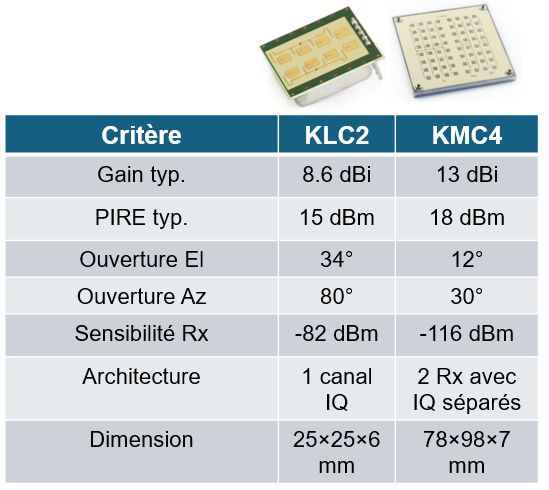
\includegraphics[width=0.5\textwidth]{src/rapport_complet/img/kmc4klc2.png}
    \caption{Tableau comparatif des caractéristiques pincipales des deux transceivers}
    \label{fig:comparatif}
\end{figure}

De plus, on dispose des diagrammes de rayonnement suivants :

\begin{figure}[H]
    \centering
    \begin{minipage}[t]{0.48\textwidth}
        \centering
        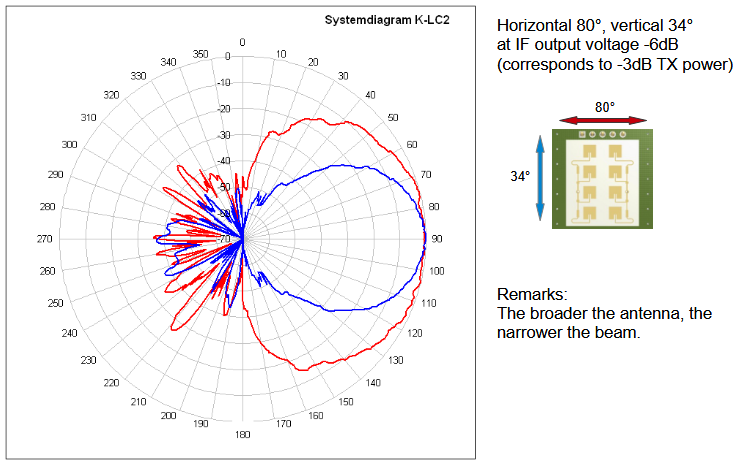
\includegraphics[width=\linewidth]{src/rapport_complet/img/diagrammeantenneklc2.png}
        \caption{Diagramme de rayonnement 2D antenne K-LC2}
        \label{fig:diagrammeantenneklc2}
    \end{minipage}
    \hfill 
    \begin{minipage}[t]{0.48\textwidth}
        \centering
        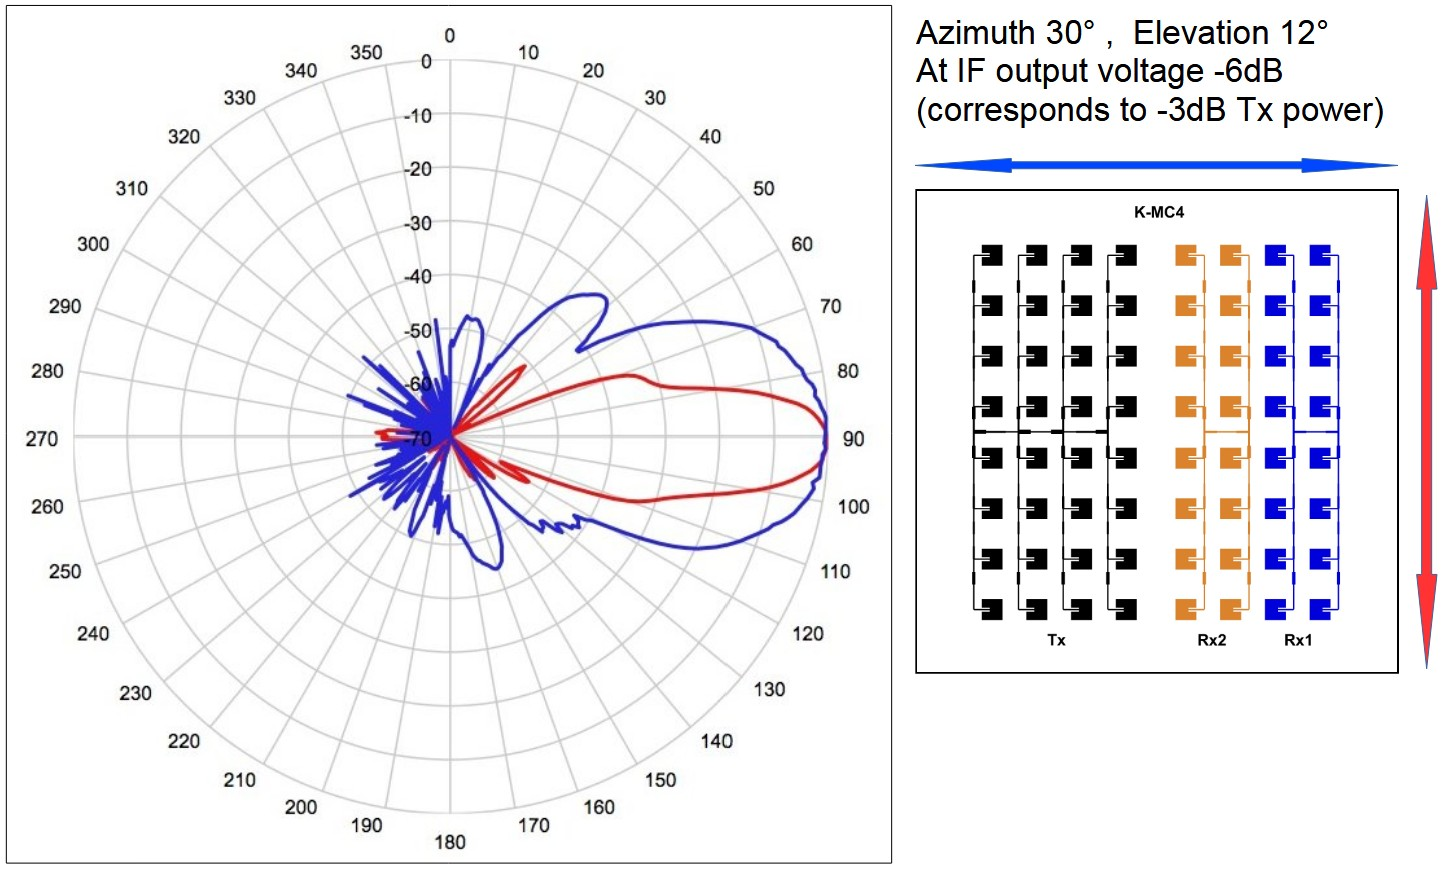
\includegraphics[width=\linewidth]{src/rapport_complet/img/diagrammeantennekmc4.jpg}
        \caption{Diagramme de rayonnement 2D antenne K-MC4}
        \label{fig:diagrammeantennekmc4}
    \end{minipage}
\end{figure}

L'architecture des deux tranceivers est sensiblement différentes. En effet, comme visible sur les figures \ref{fig:klc2synoptique} et \ref{fig:kmc4synoptique}, l'architecture du tranceiver K-MC4 est plus complexe et avancé. Permettant notamment d'obtenir via ses deux voies Rx, deux signaux IQ distincts.
Concernant la K-LC2, son architecture d'émetteur-récepteur combiné implique une isolation Tx/Rx souvent moindre contrairement à la K-MC4 avec des réseaux de patch Tx/Rx séparés physiquement pour garantir une meilleure isolation. Toutefois, cette isolation n'étant pas parfaite, et de part notre forme d'onde à émission constante, un problème de self-mixing peut apparaître.

\begin{figure}[H]
    \centering
    \begin{minipage}[t]{0.48\textwidth}
        \centering
        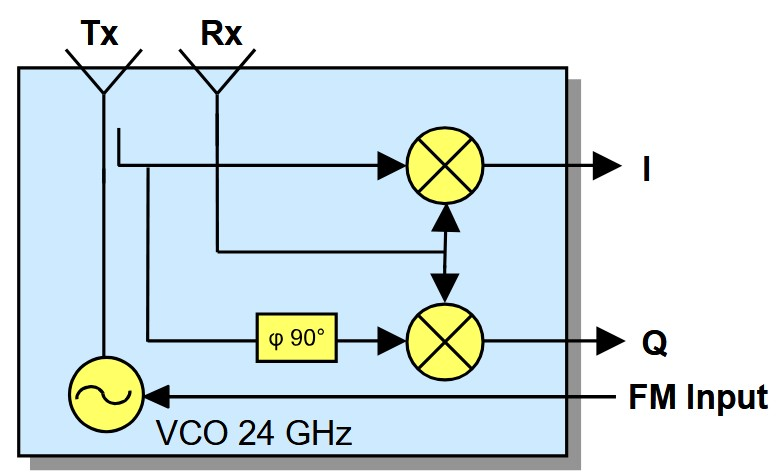
\includegraphics[width=\linewidth]{src/rapport_complet/img/klc2synoptique.jpg}
        \caption{Synoptique tranceiver K-LC2}
        \label{fig:klc2synoptique}
    \end{minipage}
    \hfill 
    \begin{minipage}[t]{0.48\textwidth}
        \centering
        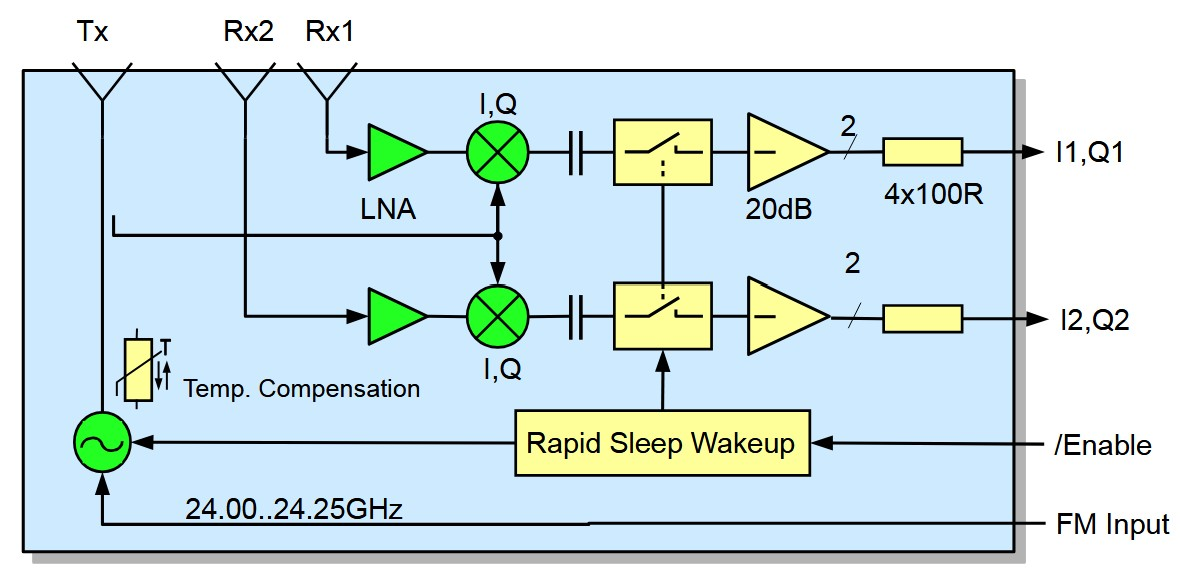
\includegraphics[width=\linewidth]{src/rapport_complet/img/kmc4synoptique.jpg}
        \caption{Synoptique tranceiver K-MC4}
        \label{fig:kmc4synoptique}
    \end{minipage}
\end{figure}

Dans un cas réel, le porteur évoluerai en extérieur et en hauteur subissant les aléats météo. C'est pourquoi, il serait nécessaire de développer un radome. Un radome est un terme dérivé de «RADar dOME ». Il s'agit d'un capot ou d'un boîtier destiné à protéger les antennes radar des influences environnementales. Chaque radome a une certaine influence sur la forme du champ de détection et la distance maximale pouvant être atteinte. Le radar peut « voir » à travers le plastique et le verre de n'importe quelle couleur. Cela permet une grande liberté de conception. Néanmoins, certaines règles doivent être prises en compte.
Le radome est un élément très important du capteur et peut avoir une influence significative sur la sensibilité, le diagramme d'antenne rayonné et l'immunité aux vibrations. La conception d'un radôme consiste à minimiser la réflexion des micro-ondes à la surface du capot. Une mauvaise conception du radôme peut même entraîner une sensibilité indésirable à l'arrière du capteur. Le matériau du capot peut agir comme une lentille et focaliser ou disperser les ondes radar. C'est pourquoi il doit avoir une épaisseur constante dans la zone utilisée pour la transmission. \cite{rfbeam_radome} Dans un premier temps, les expérimentations sont réalisées en laboratoire dans des conditions environnementales stables et propices. Ainsi, l'utilisation d'un radome sera conçue ultérieurement.

\subsubsection{Outil d'ingénierie système}
Afin de prédéterminer les performances de notre système et comparer les transceivers disponibles, un fichier Excel regroupant l'ensemble des datasheets à été mis en place. De plus, une fiche "calcul" permet de calculer les principales performances de notre système en fonction de l'environnement de test notamment :

\begin{itemize}
    \item Surface Équivalente Radar (SER) d'une cible de calibration
    \item Puissance Isotrope Rayonnée Équivalente (PIRE)
    \item Puissance réçue (équation radar)
    \item Atténuation Tx/Rx
    \item Résolution en distance
    \item Résolution en azimut
\end{itemize}

Sur la figure \ref{fig:rcscal}, quelques exemples d'expression d'estimation de la SER de cible de calibration connue.

\begin{figure}[H]
    \centering
    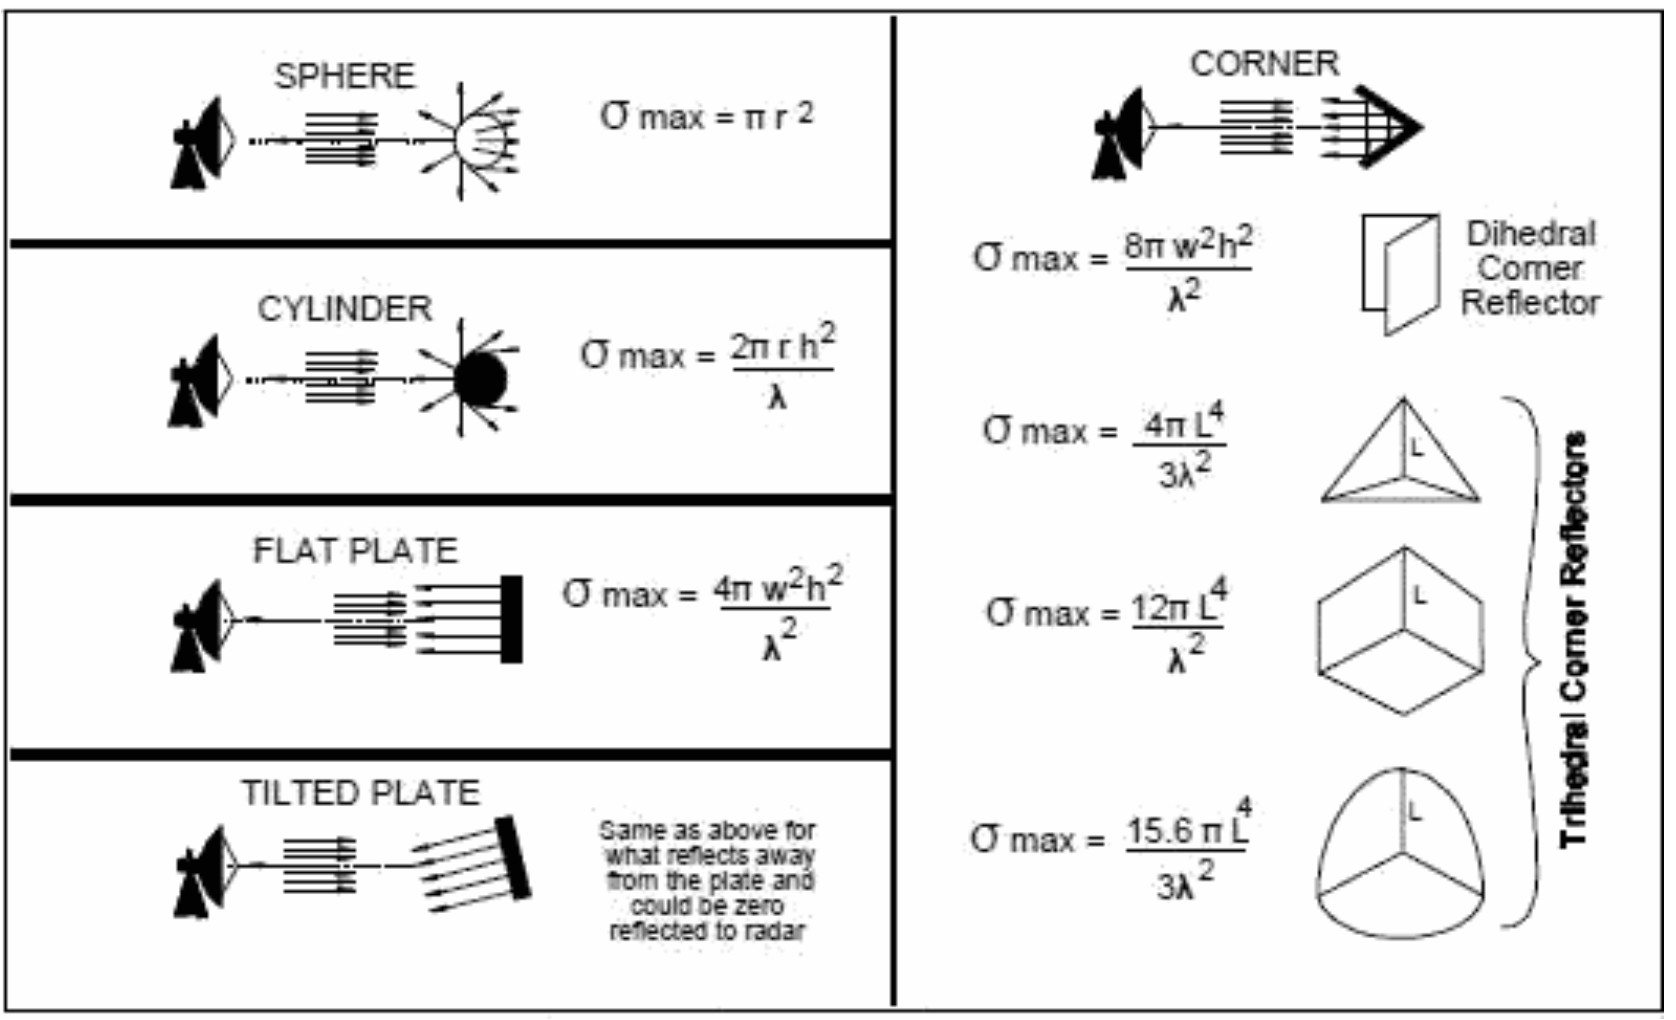
\includegraphics[width=0.8\textwidth]{src/rapport_complet/img/rcscal.jpg}
    \caption{Différentes valeurs de SER pour cibles de calibration}
    \label{fig:rcscal}
\end{figure}

\subsubsection{Définition de l'environnement de test}
\label{subsub:test}

Le premier objectif est de définir la zone "éclairée" par notre système, en fonction du setup de test en salle millimétrique. Le bras robotisé doit effectuer un balayage azimutal d'environ 1m, avec une altitude maximale fixée à H = 1,9 m. 
De plus, le phénomène de self-mixing rendant le système aveugle sur les 4 premiers mètres, une distance de fonctionnement de 5 mètres est adoptée par mesure de sécurité. 
Les distances R et Rs (cf. figure \ref{fig:tiltedtower}) sont ensuite déterminées en fonction de l'angle de dépression, l'objectif étant de respecter ces contraintes opérationnelles tout en maximisant la puissance du signal reçu.


\begin{figure}[H]
    \centering
    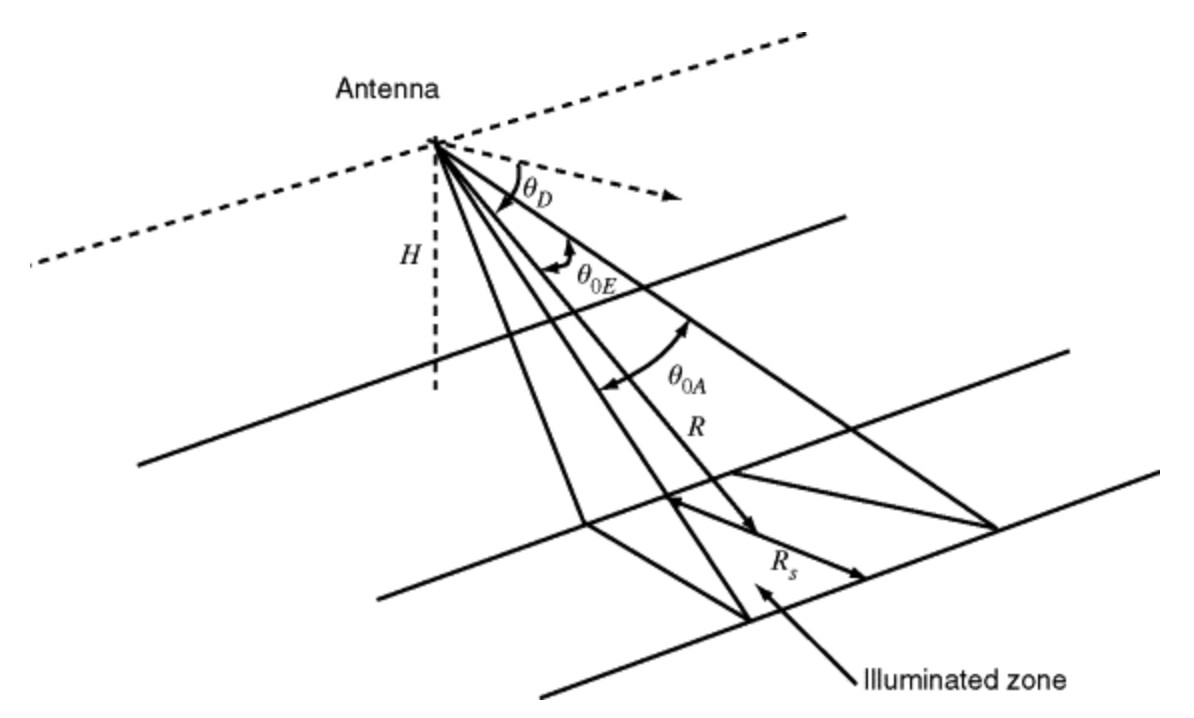
\includegraphics[width=0.8\textwidth]{src/rapport_complet/img/tiltedtower.jpg}
    \caption{Empreinte radar au sol}
    \label{fig:tiltedtower}
\end{figure}

\begin{itemize}
    \item $H$, l'altitude
    \item $\theta_D$, l'angle de dépression
    \item $\theta_{OE}$, l'angle d'élévation du faisceau
    \item $R$, la portée
    \item $R_s$, la largeur de balayage
\end{itemize}

On peut ensuite calculer :

\begin{itemize}
    \item $R = H.cosec (\theta_D)$
    \item $R_s = R.cosec (\theta_D)$
\end{itemize}

\begin{figure}[H]
    \centering
    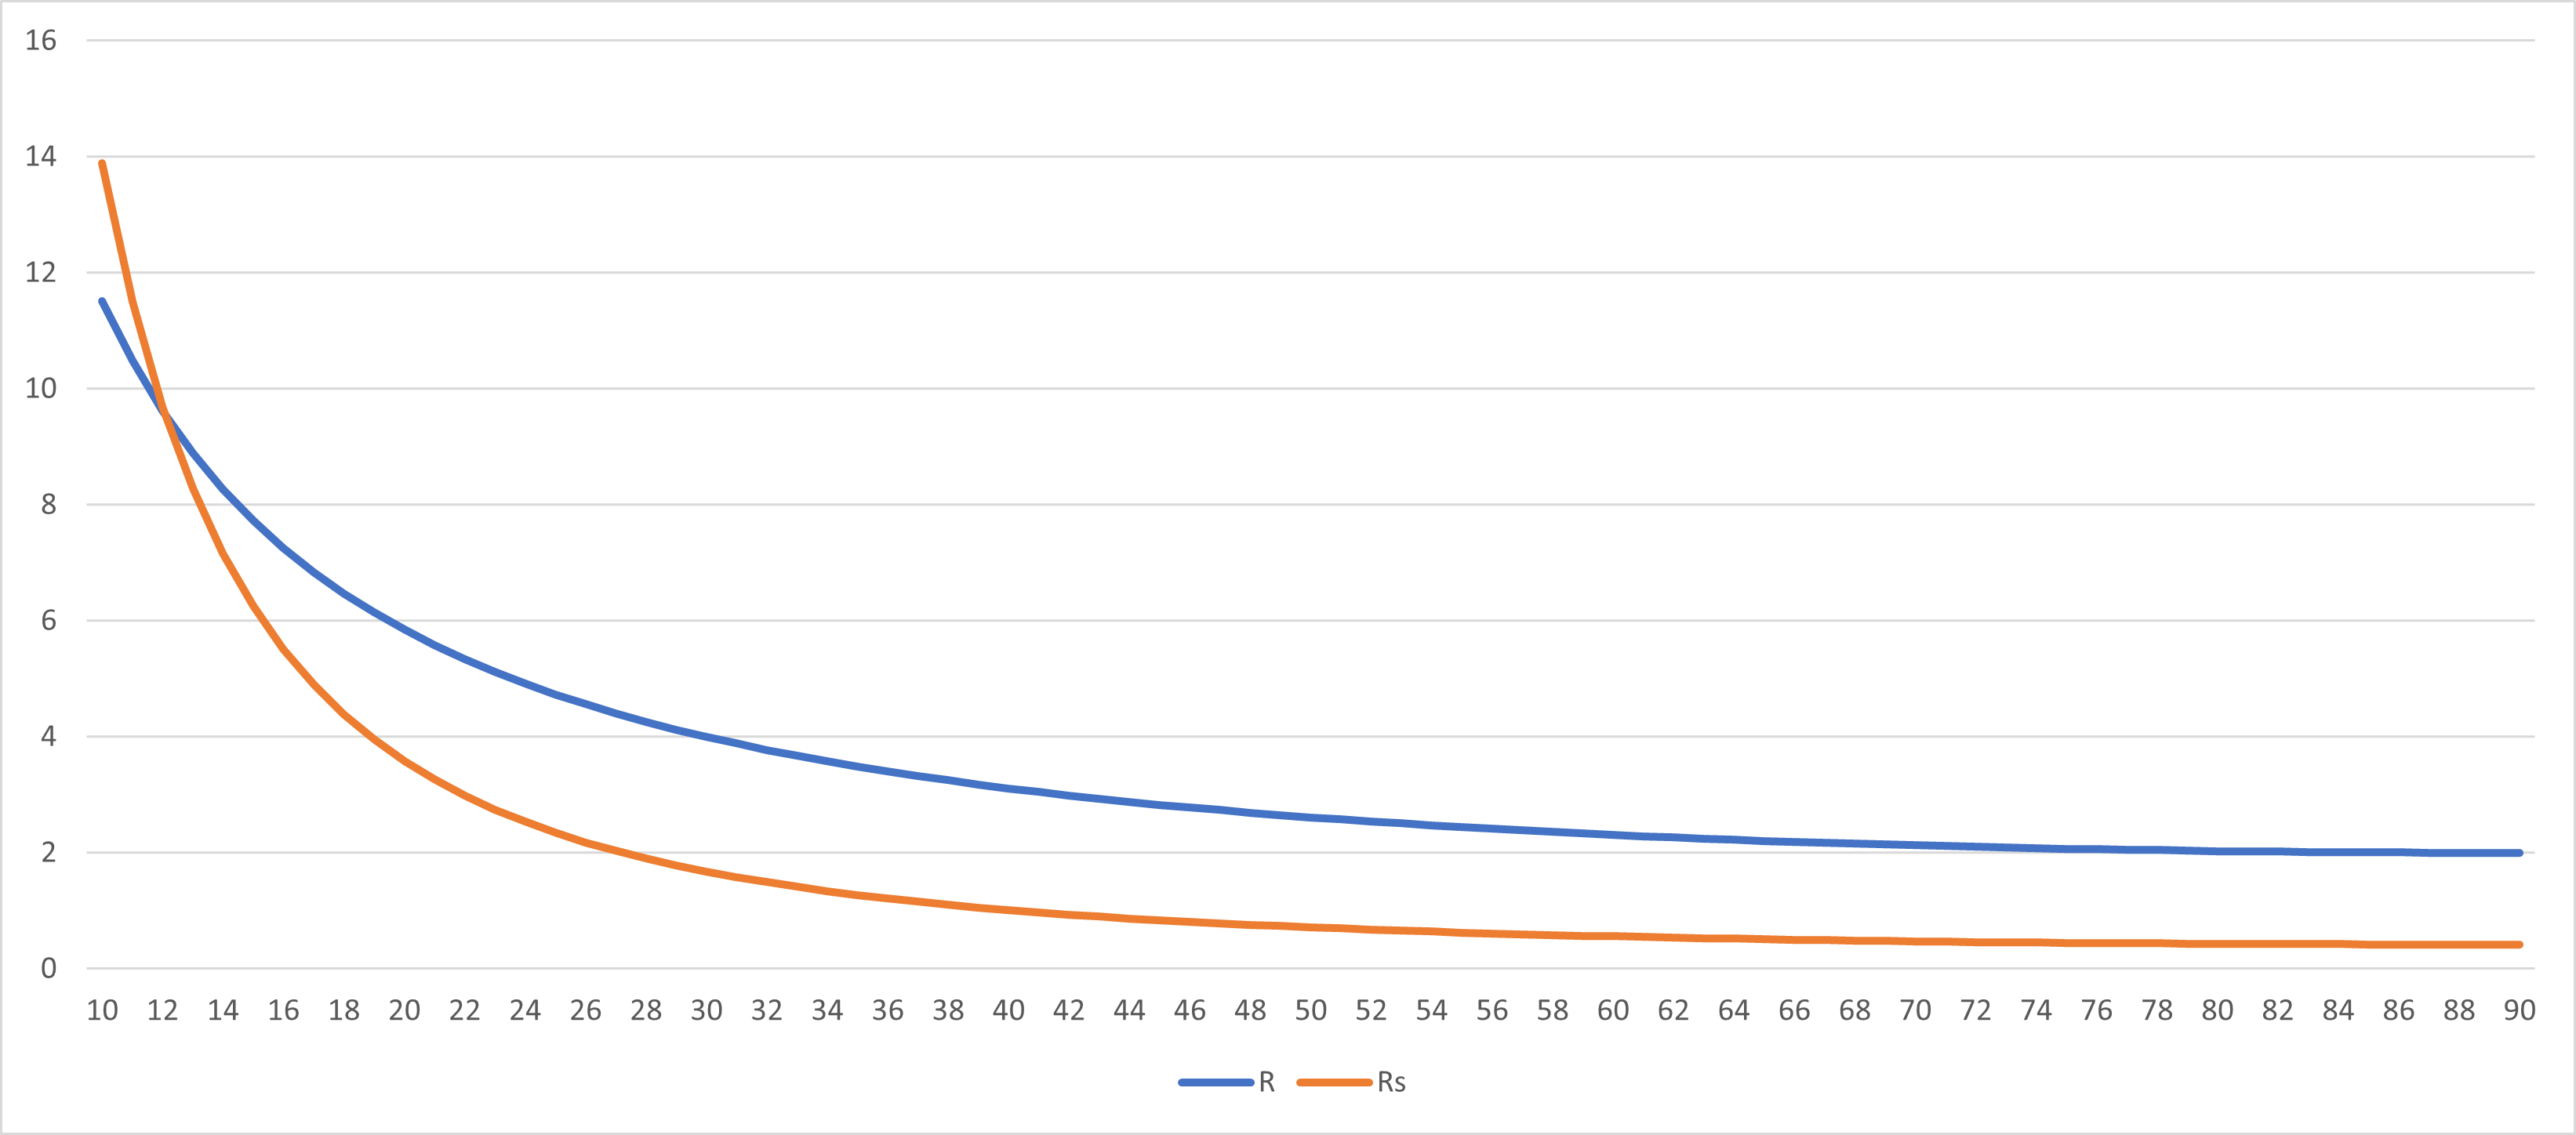
\includegraphics[width=0.8\textwidth]{src/rapport_complet/img/tilt.png}
    \caption{Zone éclairée en fonction de l'angle de dépression $\theta_D$}
    \label{fig:tilt}
\end{figure}

Le second objectif est de définir plusieurs cas de test afin de valider notre système en expérimentant plusieurs type de cibles et plusieurs taille de cibles. Ainsi, nous avons récupéré et concu (soudure plaque FR4 cuivrée) :
\begin{itemize}
    \item Sphère
    \item Trièdre, L = 15cm
    \item Trièdre, L = 10cm
    \item Trièdre, L = 5cm
    \item Trièdre, L = 2cm
\end{itemize}

On peut également estimer la puissance reçue en fonction de la hauteur du trièdre (cf. tableau \ref{fig:Prhauteurcible}). Pour rappel, la sensibilité du récepteur est donnée à -116 dBm dans la datasheet du fabricant.

\begin{figure}[H]
    \centering
    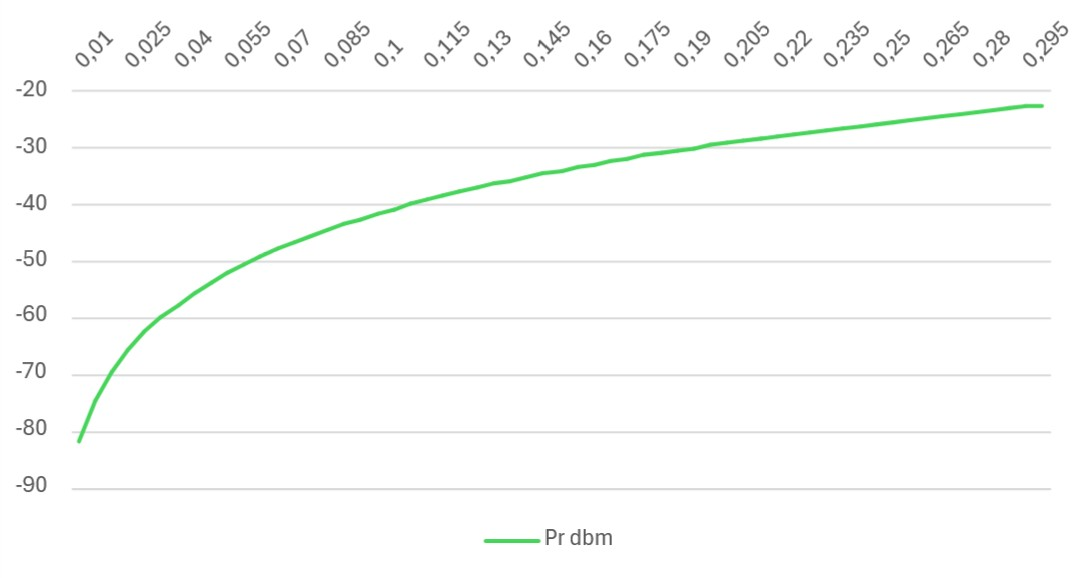
\includegraphics[width=0.8\textwidth]{src/rapport_complet/img/Prhauteurcible.jpg}
    \caption{Puissance reçue en fonction de la hauteur du trièdre}
    \label{fig:Prhauteurcible}
\end{figure}

Concernant les cas de tests, afin de différencier plusieurs cibles, nos résolutions range et azimut doivent être suffisante.
Ci-contre quelques cas de test :

\begin{figure}[H]
    \centering
    \begin{minipage}[t]{0.32\textwidth}
        \centering
        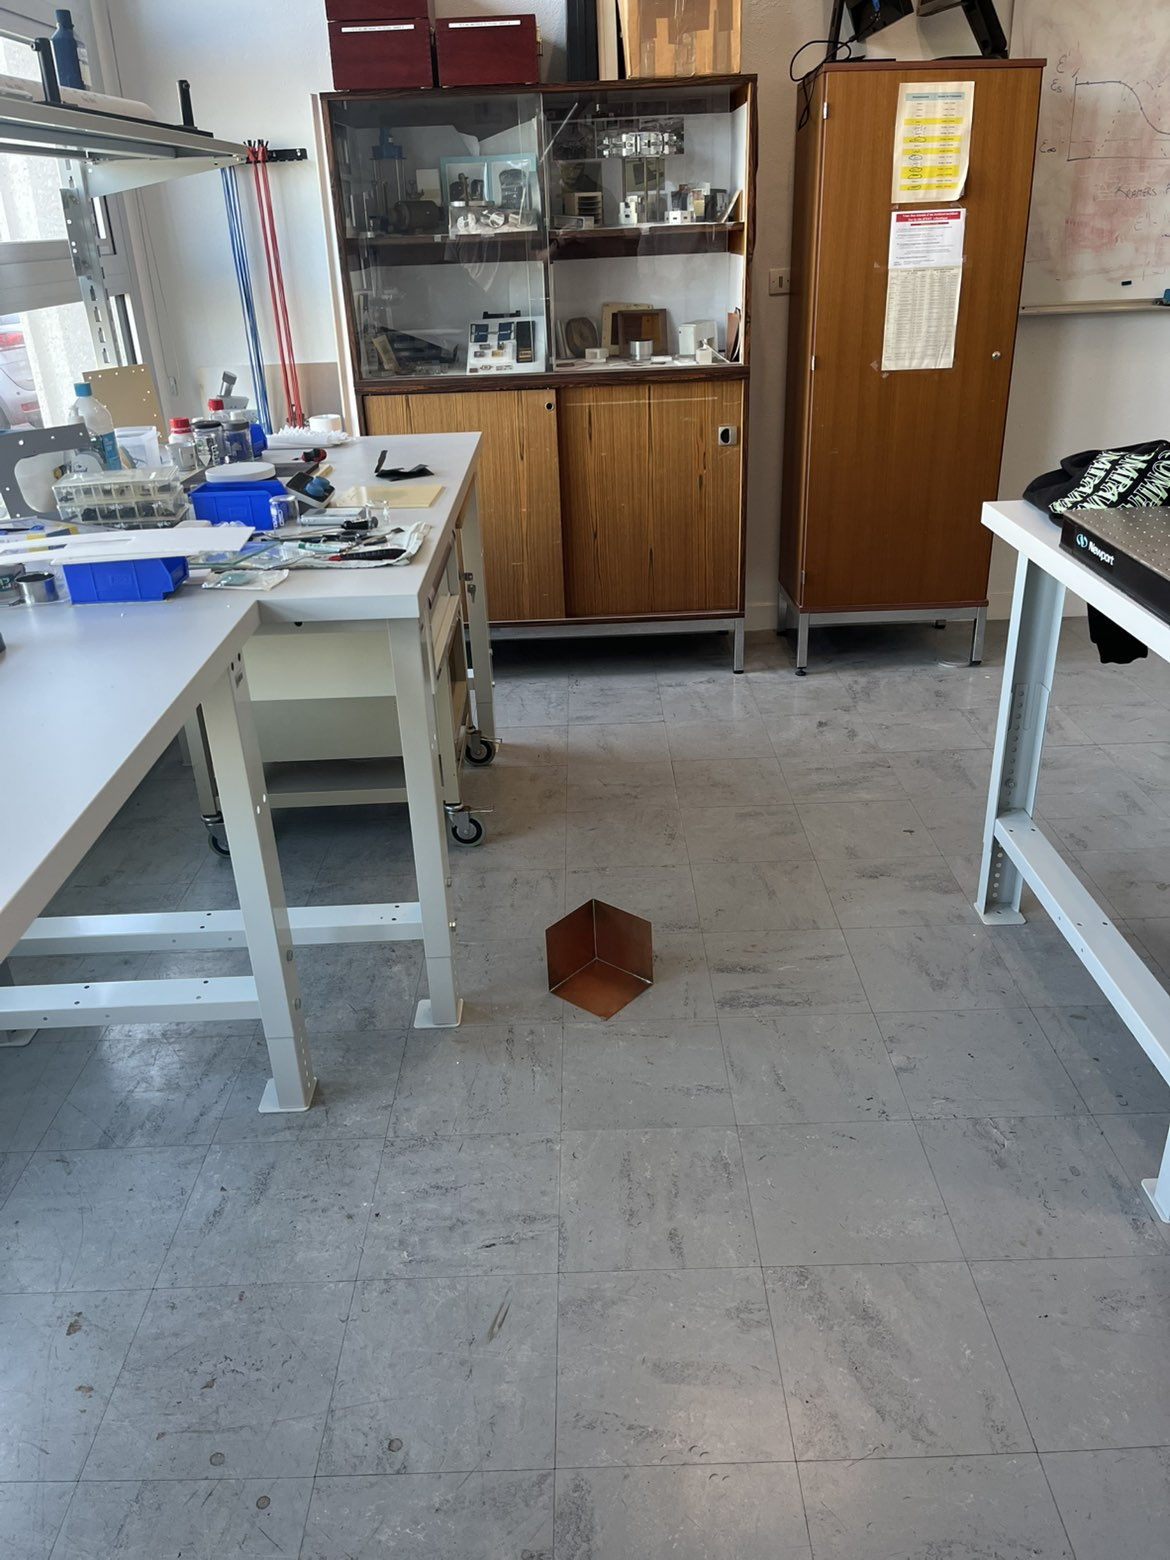
\includegraphics[width=\linewidth]{src/rapport_complet/img/grandmono.jpg}
        \caption{Monocible : grand trièdre}
        \label{fig:grand_trièdre}
    \end{minipage}
    \hfill 
    \begin{minipage}[t]{0.32\textwidth}
        \centering
        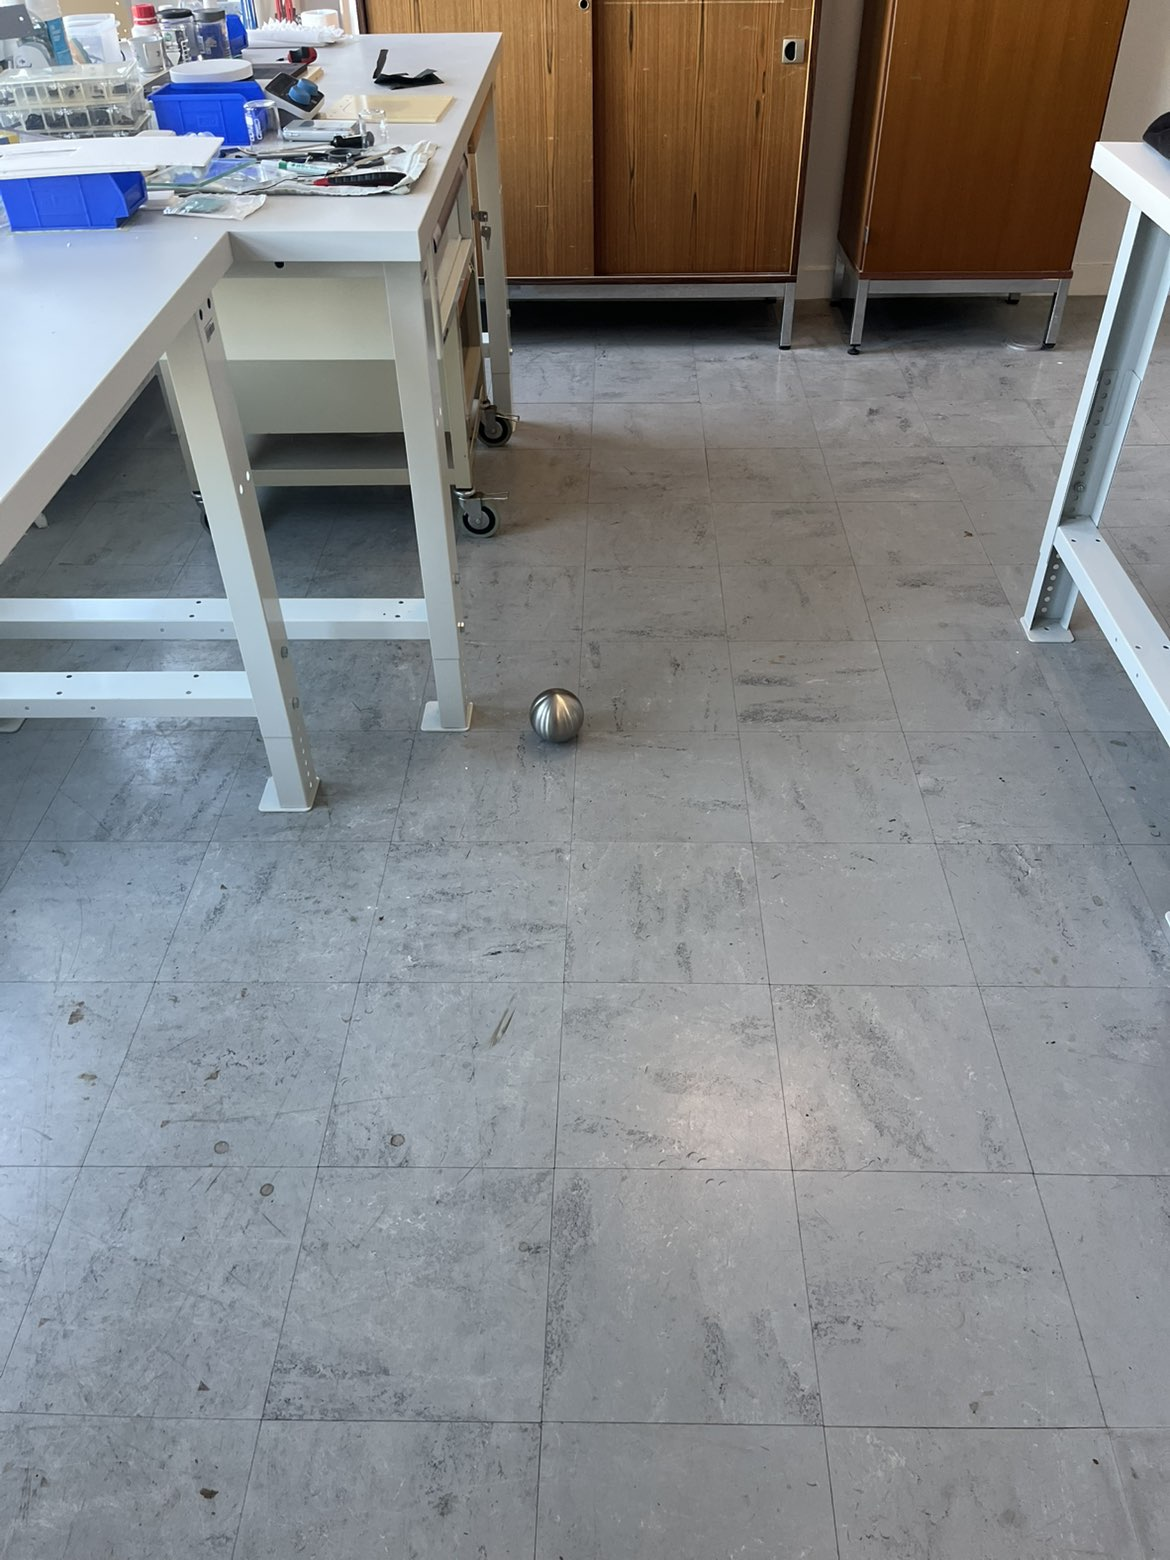
\includegraphics[width=\linewidth]{src/rapport_complet/img/sphere.jpg}
        \caption{Monocible : sphère}
        \label{fig:sphere}
    \end{minipage}
    \hfill 
    \begin{minipage}[t]{0.32\textwidth}
        \centering
        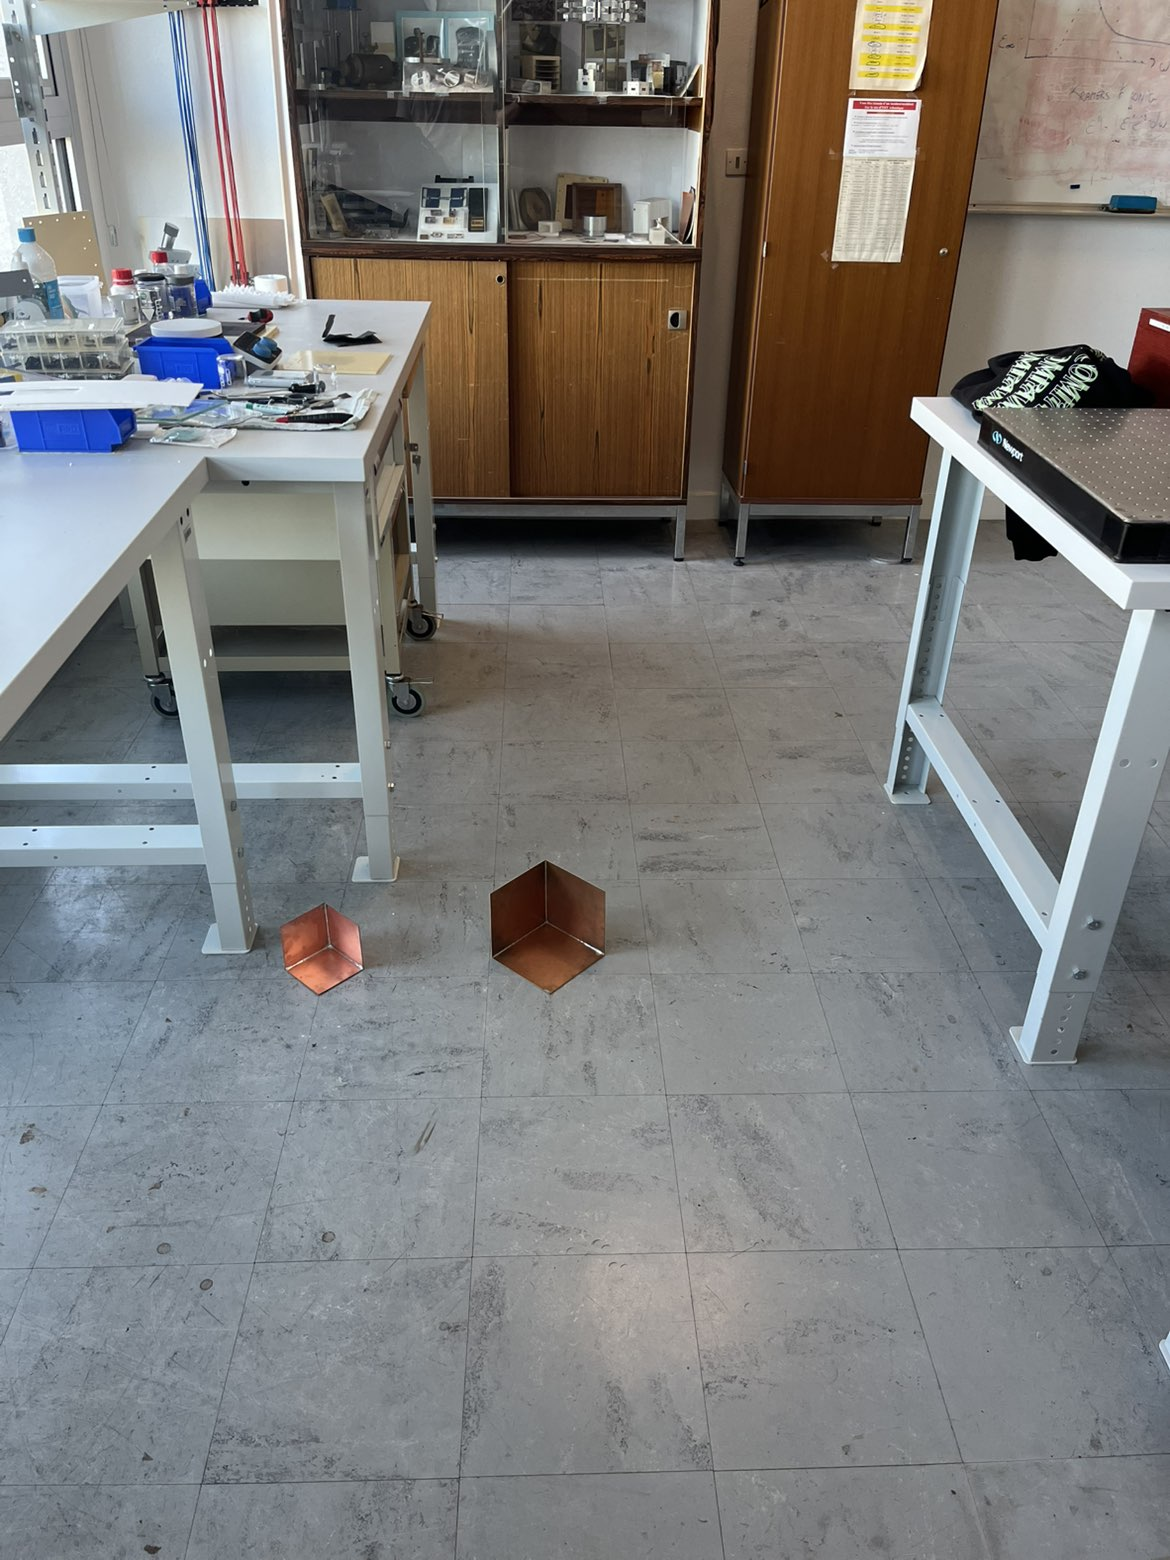
\includegraphics[width=\linewidth]{src/rapport_complet/img/multicote.jpg}
        \caption{Multicibles : grand et moyen trièdre (même range)}
        \label{fig:grand_et_moyen_trièdre}
    \end{minipage}
\end{figure}

Le bras robot est un Universal Robot 10e (cf. figure \ref{fig:bras}), contrôlable en Python, également simulé via jumeau numérique. L'ensemble de nos tests sont ainsi effectué dans la salle millimétrique C01-146A du département Micro-Ondes. Le trajet d'un mètre en azimut est effectué en 20s soit 0.05m/s afin de garantir des conditions idéales côté traitement.

\begin{figure}[H]
    \centering
    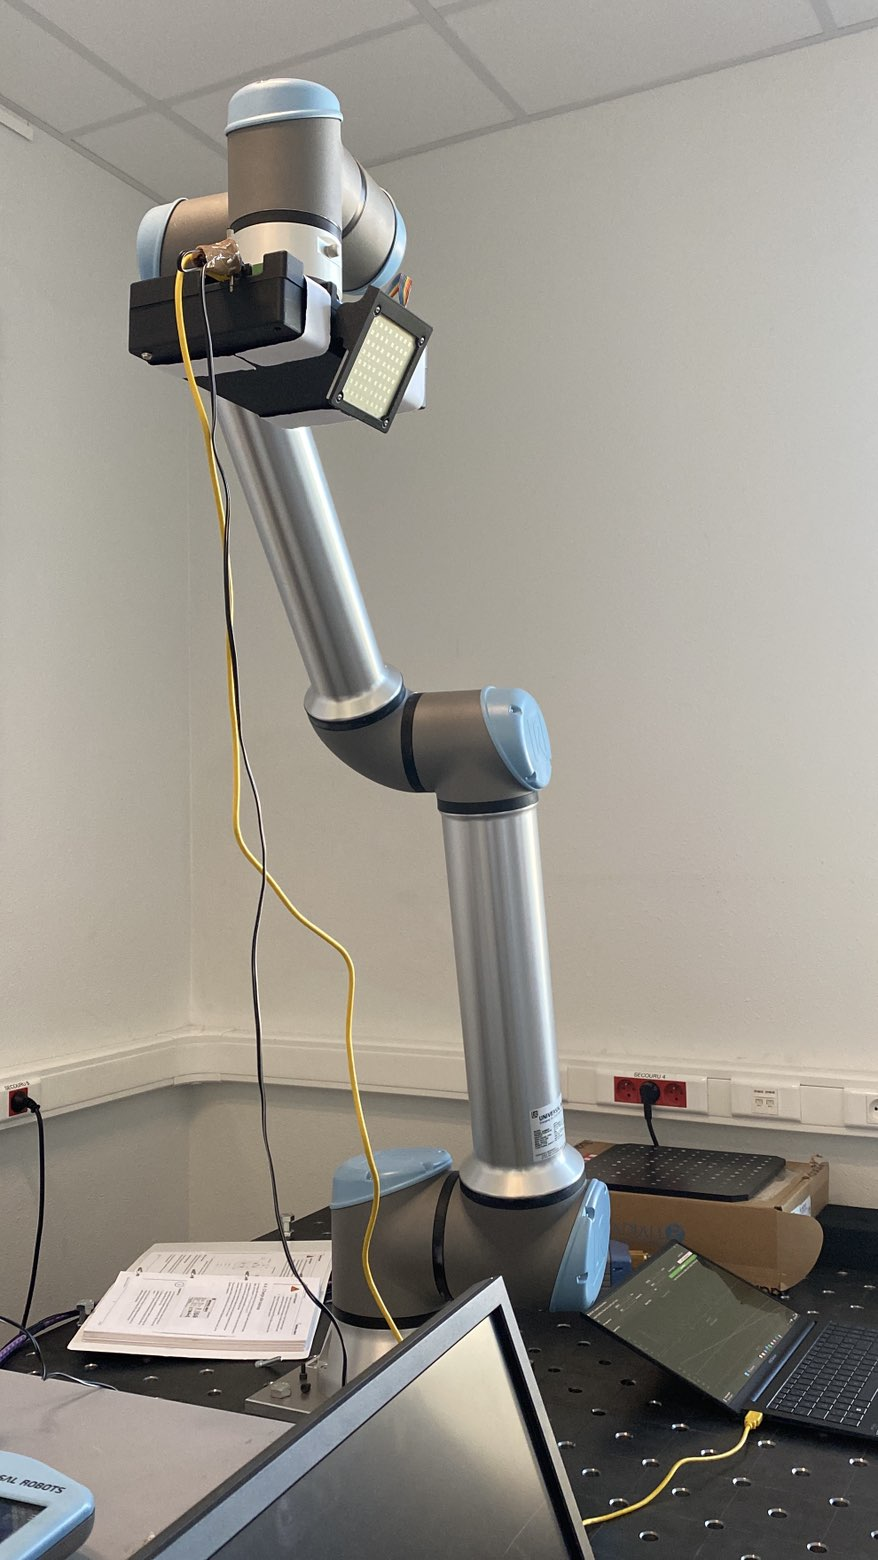
\includegraphics[width=0.5\textwidth]{src/rapport_complet/img/bras.jpg}
    \caption{Setup de test}
    \label{fig:bras}
\end{figure}




